\documentclass[10pt,a4paper]{article}

\usepackage[english]{babel}

\usepackage{libertine}
\usepackage[T1]{fontenc}

\usepackage{hyperref}
\usepackage{apacite}

\usepackage{enumitem}
\usepackage{graphicx}
\usepackage{subcaption}

\usepackage[margin=1.8cm]{geometry}

\usepackage{titlesec}
\usepackage{titling}

\usepackage{sectsty}

\usepackage{multicol}

\allsectionsfont{\centering\normalfont\sffamily\bfseries}
\renewcommand\bibliographytypesize{\small}

\setlength{\droptitle}{-10pt}
\posttitle{\par\end{center}\vskip 0.5em}
\preauthor{}
\postauthor{}
\predate{}
\postdate{}

\setlength{\parindent}{0em}
\setlength{\parskip}{0.2em}


\usepackage{gb4e}

\begin{document}

\title{\LARGE\sffamily\bfseries Linguistics Essay Writing:\\Tips, Reminders,
Suggestions}
\date{}

\maketitle

\begin{multicols}{2}

\section*{READ, THINK \& PLAN}

\begin{itemize}
  \item \textbf{Read with the essay question in mind.} Read as widely as you can,
and don’t be afraid to \textbf{skim and scan} for important or interesting
material --- it’s not always a good use of your time to absorb every paragraph
in detail. But do pay close and thoughtful attention when you home in on those
crucial sections.
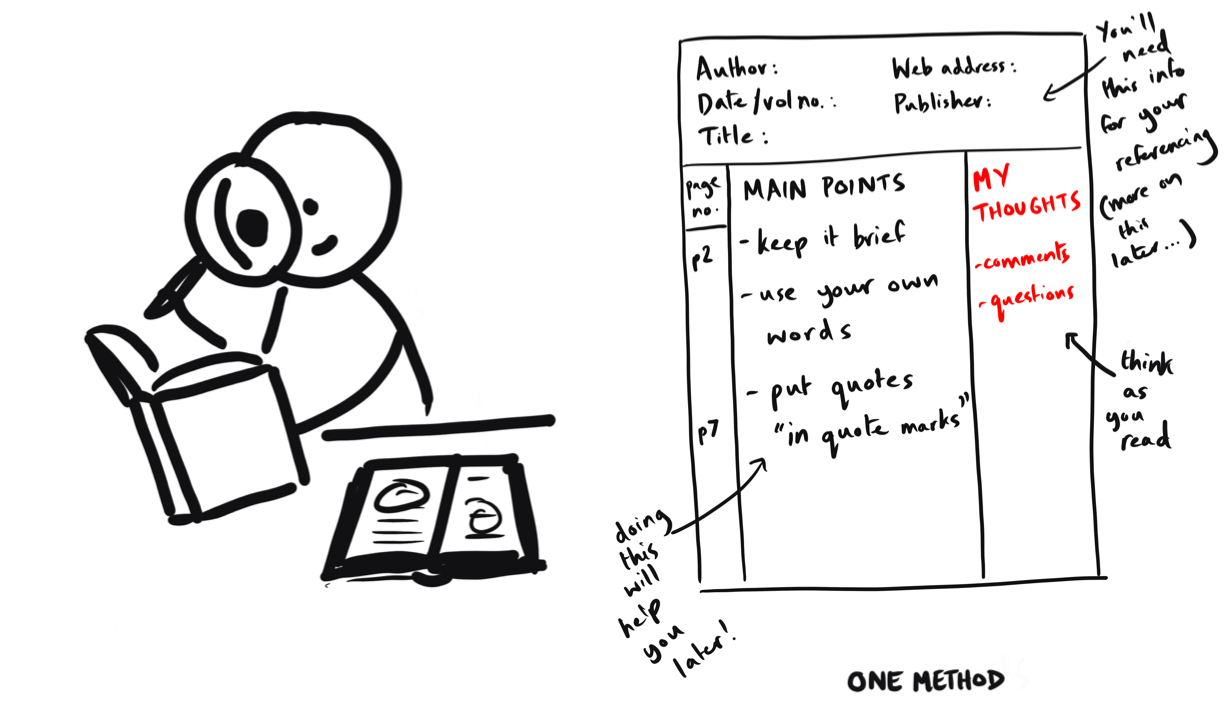
\includegraphics[width=0.9\columnwidth]{cartoons/read-take-notes.png}
  \item Take notes as you read, and consider jotting down \textbf{page numbers}
when you find a passage that might be important. This will help you when writing
and referencing later. Try to \textbf{develop a note-taking technique} that
works well for you --- some trial-and-error may be needed! Note your own
thoughts and questions as you read too.
  \item Organise your material and make an \textbf{essay plan} before you start
writing. At this stage, you might find you need to do some more reading with a
close focus on areas where you’re lacking material or feeling unsure.
  \item \textbf{Take breaks}. You probably can’t do all your reading (or write
and revise your whole essay) in a single sitting; your brain needs a chance to
absorb and consolidate the information, and your body needs a chance for other
activities. Experiment to find the work patterns and the type of breaks that you
prefer. Some people find that getting outside for a bit can be particularly
conducive to creativity and figuring out problems.
\end{itemize}

\section*{WRITE}

\begin{itemize}
  \item The first draft is always the hardest part, so adopt a non-judgmental
attitude towards your initial efforts and don’t try to edit or perfect each
sentence as you go --- \textbf{just get something written down!} If you find
yourself lacking a good example, the details of a citation, or the ideal wording
to express your idea, you might find it helps with flow if you just make a note
to come back to it and keep going. Improving on your first draft is a much less
daunting prospect once you have a good chunk of material in front of you. You
might also find that you end up cutting out some sections later, so there’s no
point in wasting time polishing them from the get-go.
  \item Avoid waffling your way through a lengthy introductory section. You
might spend a sentence or two briefly contextualising the question or laying out
what makes the topic important, but tutorial essays are short, so \textbf{get
fairly directly to the meat of your argument}. You can always review your
introduction later to see whether there’s a missing piece of background
information that would help to frame your essay.
\hspace{0.2\columnwidth}
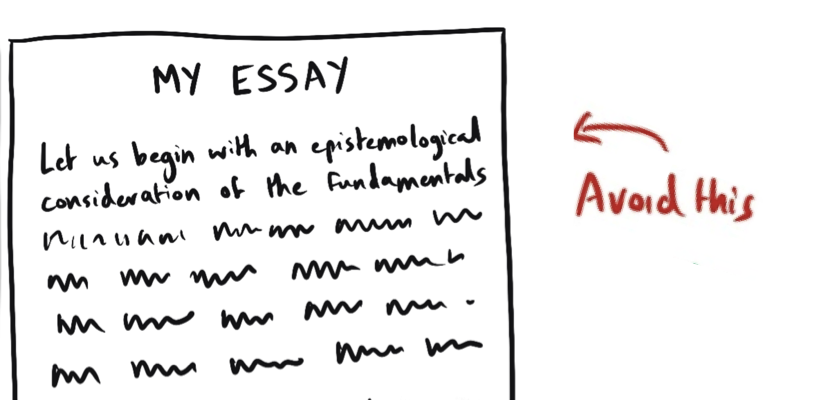
\includegraphics[width=0.8\columnwidth]{cartoons/how-not-to-introduction.png}
  \item \textbf{Concrete examples} are almost always helpful. Include them
wherever possible!
  \item Don’t be afraid to include \textbf{figures and diagrams}; they can be
very useful. If you do, make sure you refer to each figure in the main text and
explain what it illustrates.
  \item \textbf{Cite your sources}. See below for detailed advice on how to do
this.
\end{itemize}

\section*{REVIEW \& EDIT}

\begin{itemize}
  \item If you’re struggling to stay within the maximum word count, consider
whether you could \textbf{narrow the scope} of your essay a little bit to ensure
that you tackle a more focused set of ideas in the depth they deserve.
  \item When reviewing your work, pay particular attention to your concluding
paragraph(s). \textbf{Have you related your conclusion directly to the essay
question?} Have you managed to \textbf{synthesise ideas} from throughout the
main body of the essay into an overall stance \textbf{supported by the
evidence}? It’s usually best to avoid introducing new pieces of evidence as part
of the conclusion; if they’re important, find an earlier spot for them.
  \item Your essay won’t be perfect --- that’s OK! Think of each one as an
opportunity to experiment a bit, develop your writing style and your arguments,
and improve your understanding and skills. \textbf{Think about feedback} that
you’ve received on previous work --- are there any areas you need to focus on?
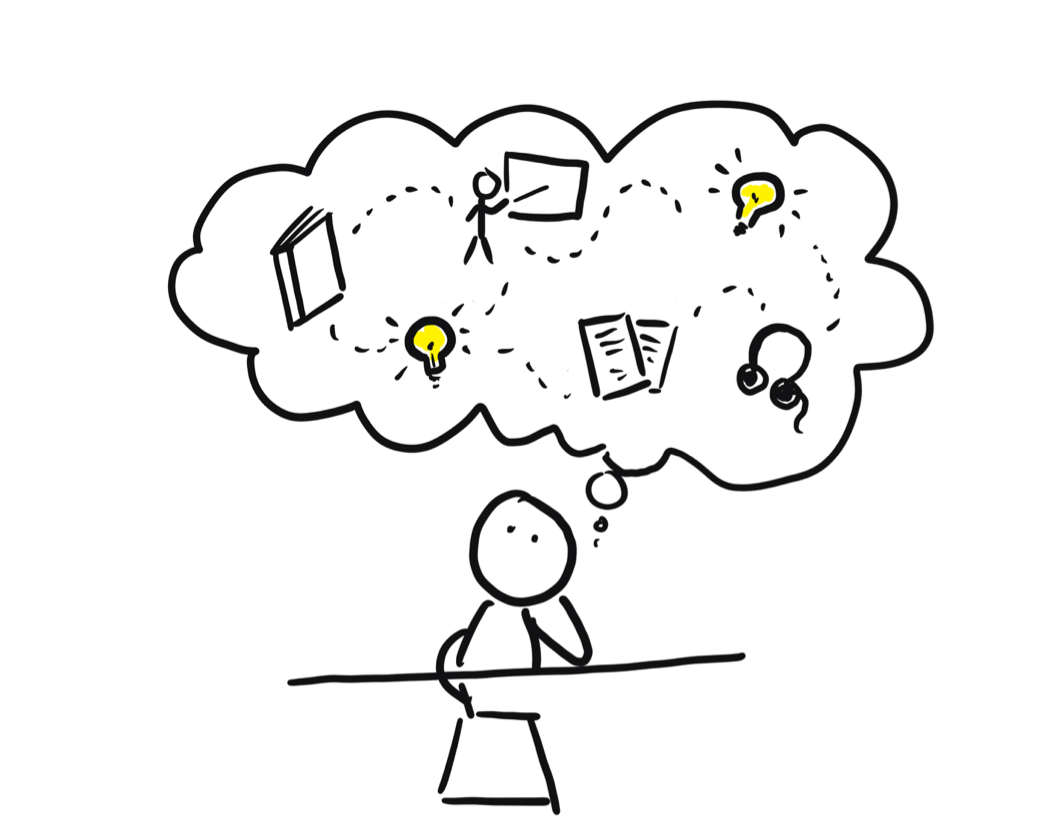
\includegraphics[width=0.9\columnwidth]{cartoons/synthesise.png}
\end{itemize}

\section*{CITATIONS \& REFERENCING}
\begin{itemize}
  \item You must include a citation wherever you refer to or make use of someone
else’s work (which you should do frequently!). This might be a
\textbf{quotation} (in which case you should make it clear that you are quoting
directly), a \textbf{paraphrase} in your own words, or a general mention of a
\textbf{main idea or finding} that they have put forward.
  \item You’re free to use any consistent format for referencing (unless your
tutor asks for something specific), but it should have two components: 1) a
\textbf{citation at the relevant point in the text}; 2) a \textbf{bibliography /
reference list} at the end of your essay containing all the works you have
referred to.
  \item If you’re not sure how to format your citations, a recommended option
is to aim for
\href{https://apastyle.apa.org/style-grammar-guidelines/references/examples}
{\textbf{APA style}}, on which you can find lots of helpful articles and
information online. Don’t worry too much about the fussier details --- just use
it as a guide and aim to be consistent!
\end{itemize}
\vspace{0.05em}

{\centering
\hspace{10pt}
\fbox{
\begin{minipage}{0.9\columnwidth}
  {\small
\textbf{APA Style Referencing: An example text}

\vspace{5pt}
The Jabberwock is widely regarded as an alarming creature \cite<see>[for a
review]{carroll71}. \citeA{queen41} note that even unusually fast runners will
fail to keep up with this particular foe,
but there is debate over whether its attacks are more likely to take the form
of `rattle theft' \cite[p.96]{dum52} or semantic equivocation
\cite{humpty63}. It is clear, however, that challenging the monster without
 adequate dietary hay intake is likely to be a mistake \cite{knight50}.
 Combatants should also take care to divide a loaf by a knife before commencing
 their attack \cite{queen41}.

\vspace{5pt}
\textbf{References}
}
\tiny{
\bibliographystyle{apacite}
{\def\section*#1{}
\bibliography{bib.bib}
}
}
\end{minipage}
}
}


\section*{PRESENT YOUR WORK}

\begin{itemize}
  \item	Feeling techy and/or keen for some typesetting nerdery? You might have
fun experimenting with
\href{https://en.wikibooks.org/wiki/LaTeX}{\textbf{\LaTeX}}. It's especially
great for things like IPA symbols, linguistic examples with glosses, syntax
trees, and formatting your references.
  \item	Before submitting your work, check whether any particular
\textbf{formatting style} (e.g. double-spaced text) or file type (e.g. PDF) is
required. Don’t forget to put your name on there somewhere!
  \item Make sure you have \textbf{a copy of your essay} in front of you for the
tutorial. You might want to give it a quick \textbf{re-read beforehand} to
refresh your memory of the topic.
\end{itemize}

\end{multicols}

\begin{figure*}[h!]
\fbox{
\begin{minipage}{\textwidth}

\section*{SUMMARY OF TIPS}
\begin{multicols}{3}
  \begin{itemize}[noitemsep]
      \raggedright
      \sffamily{
      \item	Read widely, use skimming and scanning
      \item	Take notes, including page numbers
      \item	Make an essay plan
      \item	Take breaks while working
      \item	Don’t get psyched out: bash out that first draft, however rough!
      \item	Keep the introduction short
      \item	Include concrete examples
      \item	Use figures/diagrams if helpful
      \item	Cite your sources
      \item	Narrow the scope if you’re short on space
      \item	Relate your conclusion directly to the question
      \item	Synthesise ideas presented throughout
      \item	Think about how to apply previous feedback
      \item	Check the formatting
      \item	Re-read before the tutorial
      }
    \end{itemize}
    \centering
    
\includegraphics[width=0.23\columnwidth]{cartoons/grad.png}
\end{multicols}
\end{minipage}}
\end{figure*}

\footnotesize{
\textit{Document produced by Emily Darley, Language \& Brain Lab, University of
Oxford, with illustrations by Emily Downes. Feel free to share or link to
this. \\
Questions, comments, or suggestions for this document? Email}
\texttt{emily.darley@ling-phil.ox.ac.uk} \textit{or submit a pull request at}\\
 \href{https://github.com/emilyjdarley/essay-writing-guide}
 {\texttt{https://github.com/emilyjdarley/essay-writing-guide}}\textit{.}}
\end{document}
